\chapter{2020-06-23}

\textbf{Check List}
\begin{enumerate}
    \item \faCheckSquareO Figure out why `NAN' appears during training. \\
        A: the scores for some relation types are too small and caused the underflow when apply log function to them. A small number $\epsilon =1e-9$ is added to the scores for numerical stable.
    \item Debug the relation classifier \\
    For now, when $\beta_1$ is increased, the relation prediction accuracy become higher, but the alignment and completion performances dropped.  Try to figure out why, the code problem or the idea problem?
    Try to make the model and task to be simple to debug the relation classifier. 
    \begin{enumerate}
        \item \faCheckSquareO Try simpler version of dataset, e.g., two relaiton types.
        \item Observe some prediction outputs for alignment rank, completion rank, and relation prediction (both training and valid). 
    \end{enumerate}
    
    \item Relation classification overfitting: try different training strategy to alleviate the problem. 
    \begin{enumerate}
        \item \faCheckSquareO Play with hyperparameters: lr, batch\_size, and training\_epoch. 
        \item \faCheckSquareO Pretrain the relation classifier.
        \item \faCheckSquareO Train the relation classifier every K ($K$ \textgreater $1$) epoch instead of every epoch. 
    \end{enumerate}
\end{enumerate}

\section{Train 2 relation types}
When I was doing the experiments of learning only two relation types and visualizing the correlations between rel-acc and other metrics (hits@N, mr, mrr), I noticed that the prvious conclusion: ``\textbf{when rel-acc goes up, the other metrics go down}" is not completely correct (see Figure~\ref{fig:iptranse_C_S_V7_lineplot_metrics}). The  vibration at high rel-acc is because of more datapoints. From these curves, we can see when rel-acc is high, the other metrics could either high or low. It seems that there is no positive relationships between rel-acc and other metrics. 
Although I haven't figure out why, it gives me a hint that I can train them separately. %That is, we can first train the relaiton classifier to reach a decent rel-acc, and then reduce the frequency of updating parameteres in relation classifier. 
So, I made the following modifications for training the relation classifier:
\begin{enumerate}
    \item Separate the training process of 1) learning entity and relation embedding matrices, and 2) learning relation types. Then two optimizers are used to train two parts separately (previous: losses are added into one total loss and train it with one optimizer.)  
    \item The relation classifier is trained along with the embedding matrices at first N epoches. After that, it's updated every K epoches to avoid overfitting. This can ensure the relation classifier is well trained and also reduce the overfitting problem (see Algorithm~\ref{algo:asynchronously_training}).
\end{enumerate}

    The key difference is the gradients from the margin loss $L_e$ for triples  (see Figure~\ref{fig:model_architecture}) to the parameter $\theta$ in the relation classifier are cut down. So $\theta$ is only updated by $L_r and L_p$. 

\begin{algorithm}[H]
    \SetAlgoLined
    \KwIn{Triples from ConceptNet and SWOW}
    \KwIn{Aligned entity seeds}
    \KwIn{$N, M$ signify the max trining epoch for $L_e$ and $L_{rp}$, $N \geq M $. $K$ denotes an int number.}
    \KwResult{Entity embedding matrix $\mathbf{E}$, relation embedding matrix $\mathbf{R}$}
    \KwResult{Relation type classifier with parameter $\theta$}
    %$L_{rp} \gets \beta_1*L_r + \beta_2*L_p$\;
     initialization\;
     \For{$i \gets 0$ \textbf{to} $N$} {
            \eIf{$i < M$} {
                Update $\theta$
            } {
             \If{$ i \geq  M \vee i \% K =0$} {
                Update $\theta$ } 
            }
                Update $\mathbf{E}, \mathbf{R}$
      }
    \caption{\label{algo:asynchronously_training} Asynchronously trainining embedding matrices and relation types}
    \end{algorithm}

    \begin{figure}[!ht]
        \centering
        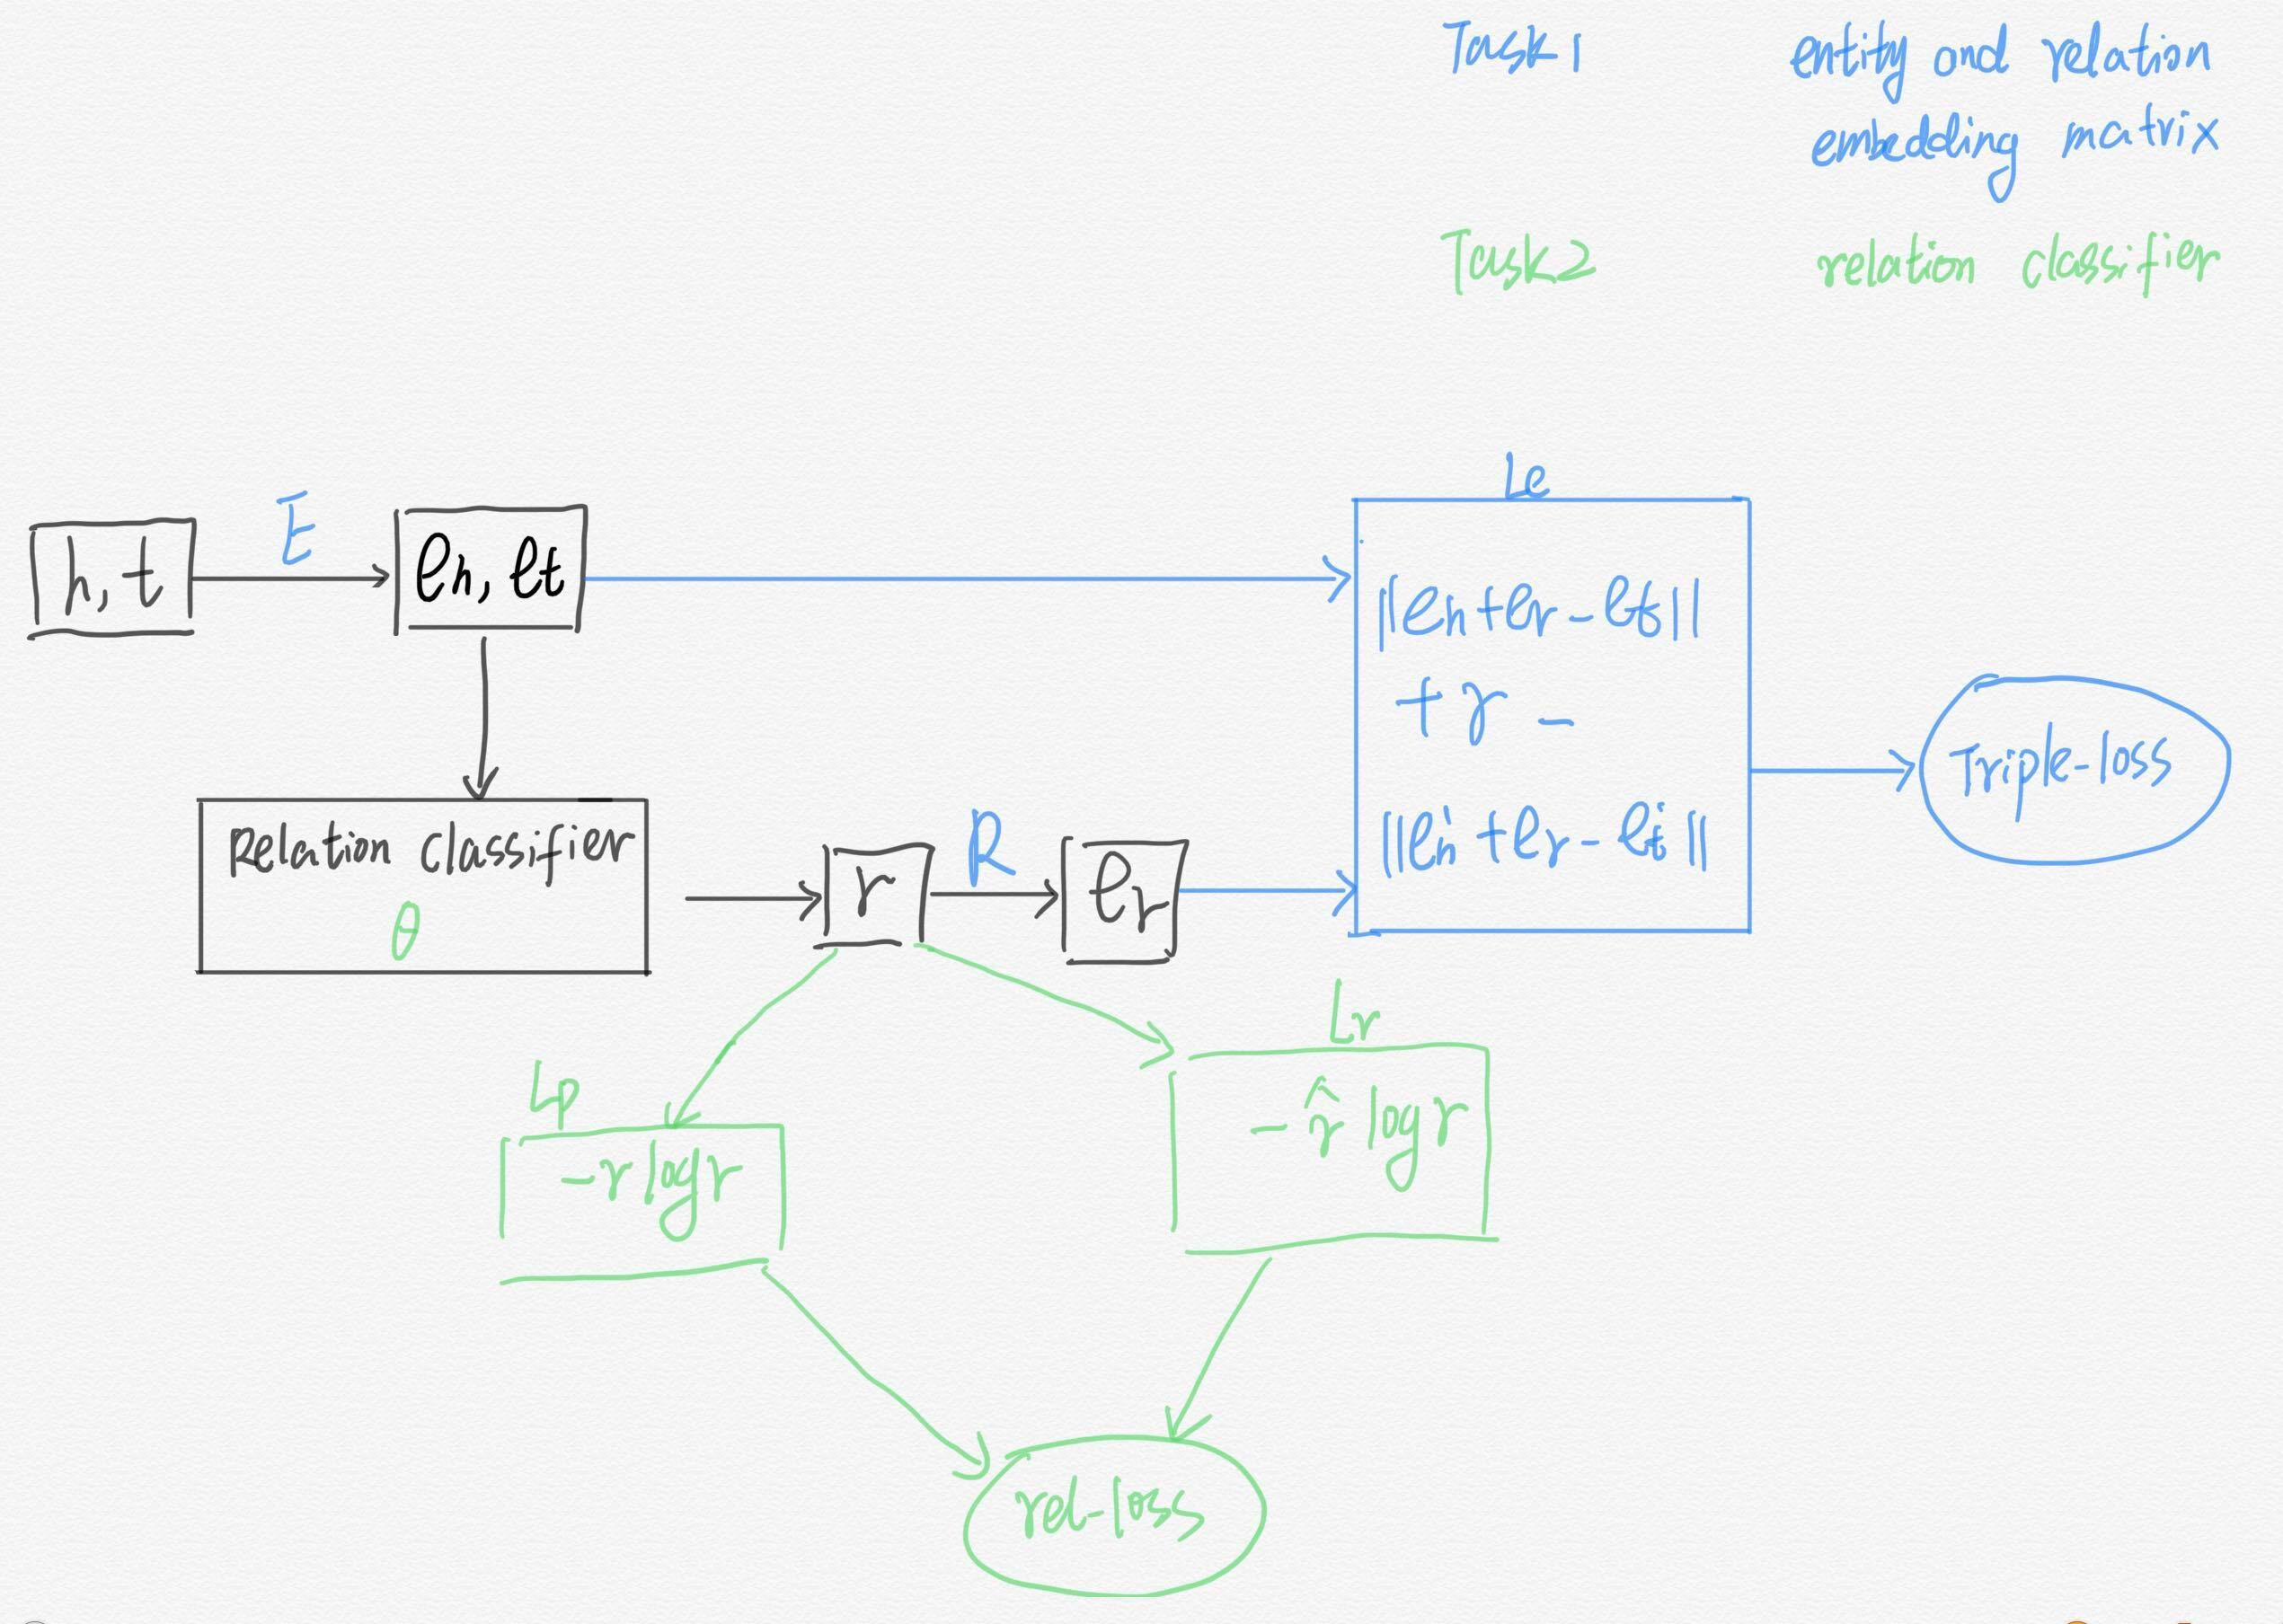
\includegraphics[width=\linewidth]{0623/model_architecture.jpg}
        \caption{\label{fig:model_architecture} The data flow in the model.}
    \end{figure}
\begin{figure}[H]
    \centering
    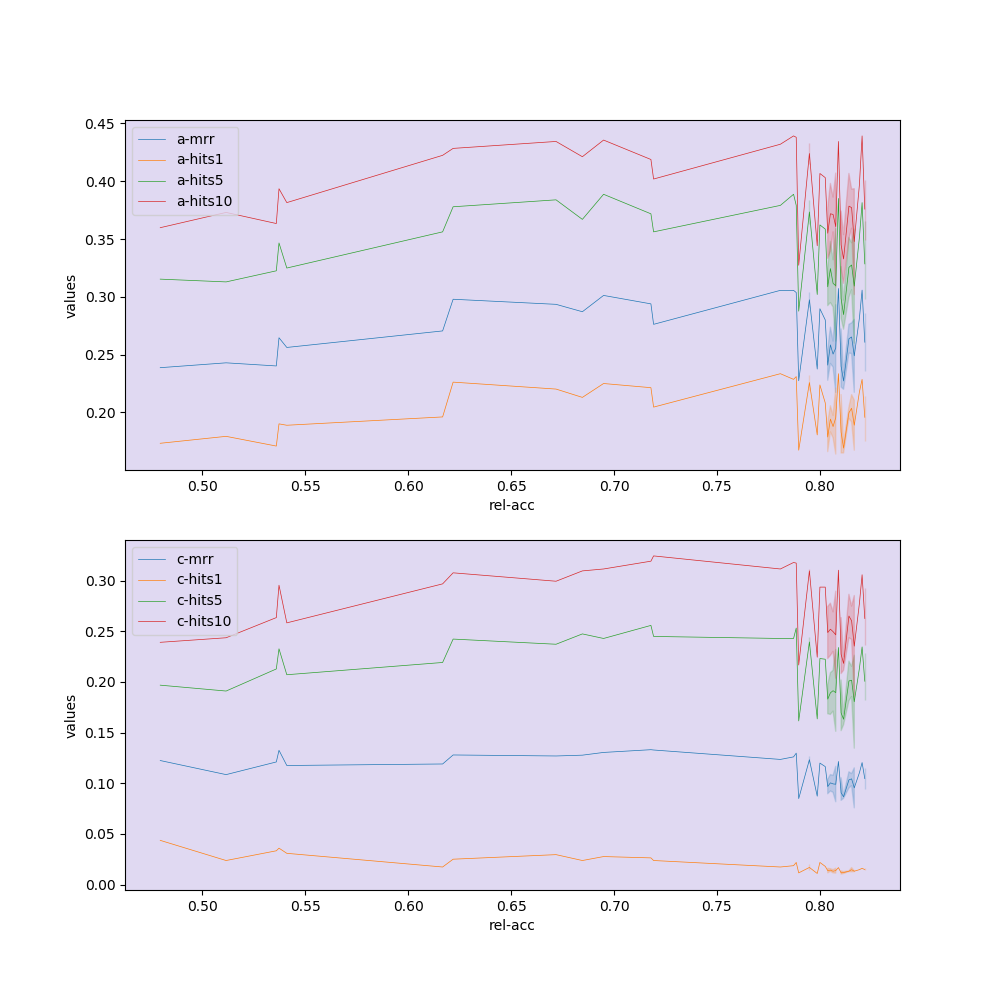
\includegraphics[width=\linewidth]{0623/iptranse_C_S_V7_lineplot_metrics.png}
    %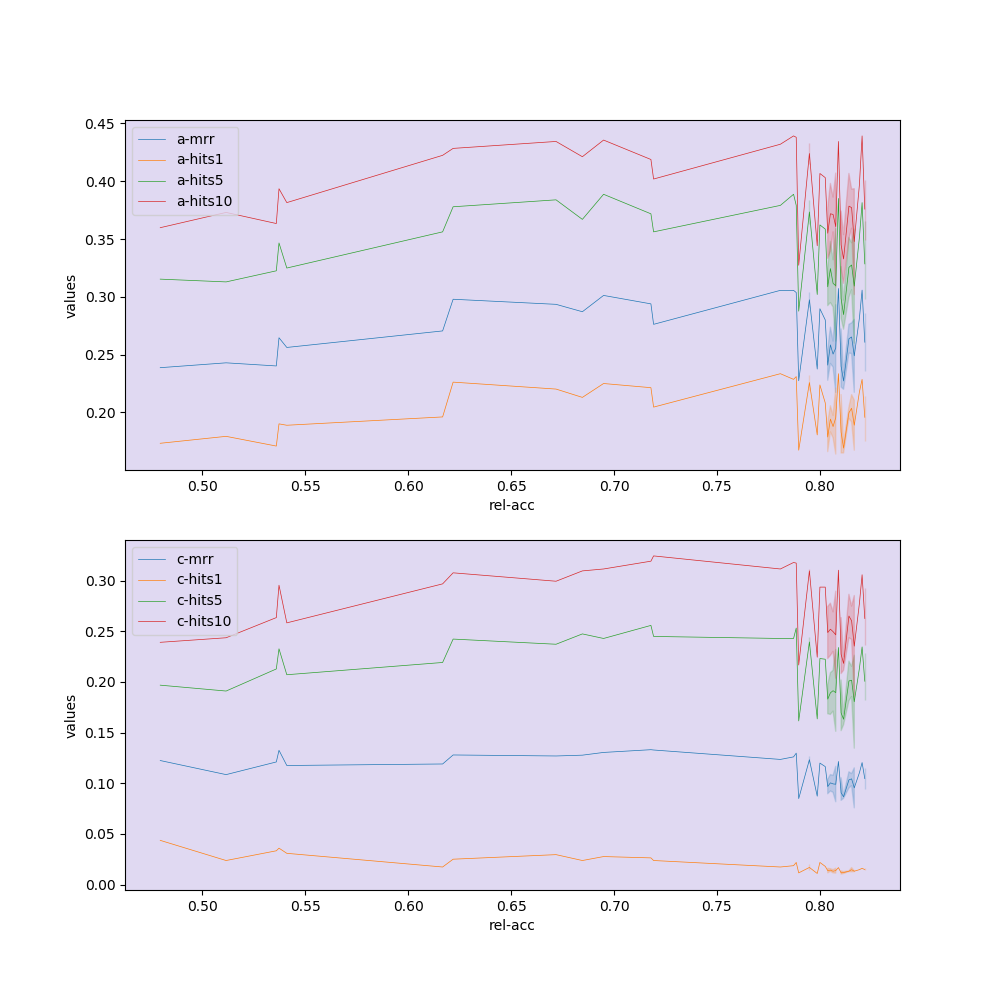
\includegraphics[scale=0.5]{0623/iptranse_C_S_V7_lineplot_metrics.png}
    \caption{\label{fig:iptranse_C_S_V7_lineplot_metrics} Correlations between rel-acc and other metrics. Embedding matrices and relations types are optimized with one optimizer. Parameters in relation classifier are updated with embedding matrices at every epoch.}
\end{figure}

\begin{figure}[H]
    \centering
    %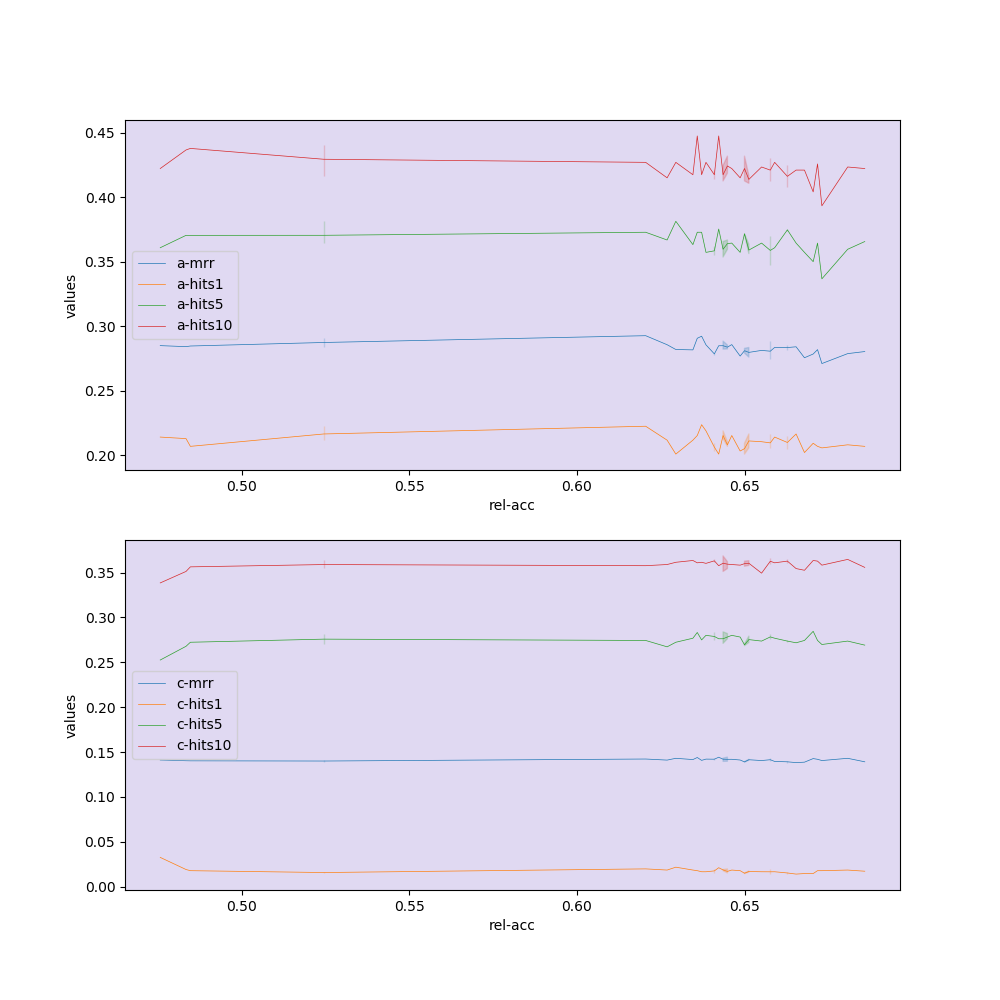
\includegraphics[scale=0.5]{0623/iptranse_C_S_V7_0621_lineplot_metrics.png}
    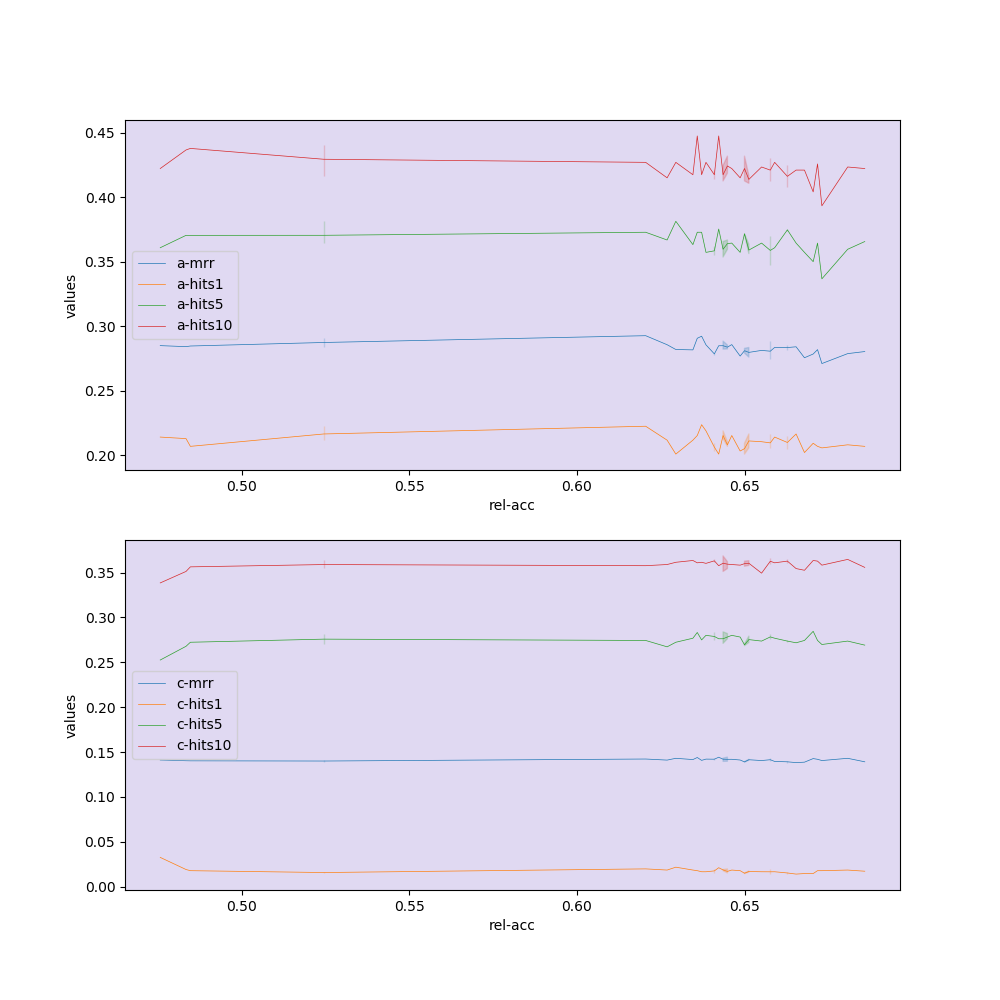
\includegraphics[width=\linewidth]{0623/iptranse_C_S_V7_0621_lineplot_metrics.png}
    \caption{\label{fig:iptranse_C_S_V7_0621_lineplot_metrics} Correlations between rel-acc and other metrics. Embedding matrices and relations types are optimized with two optimizers. Parameters in relation classifier are updated at first 100 epoches and then updated every 30 epoches in the remaining 900 epoches. Embedding matrices are updated at every epoch. The vibration is reduced compared with Figure~\ref{fig:iptranse_C_S_V7_0621_lineplot_metrics} and also the values of other metrics increased slightly. However, the average relaiton accuracy also dropped from 0.80 to 0.65 (underfitting). So in the next section, I tried to use less dropout rate and increase the learning rate and the hidden dimensions of relation classifier.}
\end{figure}
\clearpage

\section{Train 34 relation types}

Using similar startegy described as above. I run the model on the dataset with 34 types relations. Results are shown in Figure~\ref{tab:asynchronously_training_results}.
We can see the good news is the the overfitting problem is solved and the balance between rel-acc and other metrics is decent. When increasing the rel\_hidden\_dim from 100 to 500, the rel-acc also increases. 

One problem I observed from Figure~\ref{fig:asynchronously_training_results_curves} is that the vibrations of these loss curves are very strong (see the backgrounds of three losses.) They are decreasing overall, but not very stable. This could suggest that the leraning rate is too large, I should try to lower it. However,  the curves of metrics (Figure~\ref{fig:asynchronously_metrics_results_curves}) show lowering the learning rate also cause the dropping of performances. May be I could use a large learning rate at the beginning and a small one in the later phase. 


\begin{figure}[!ht]
    \centering
    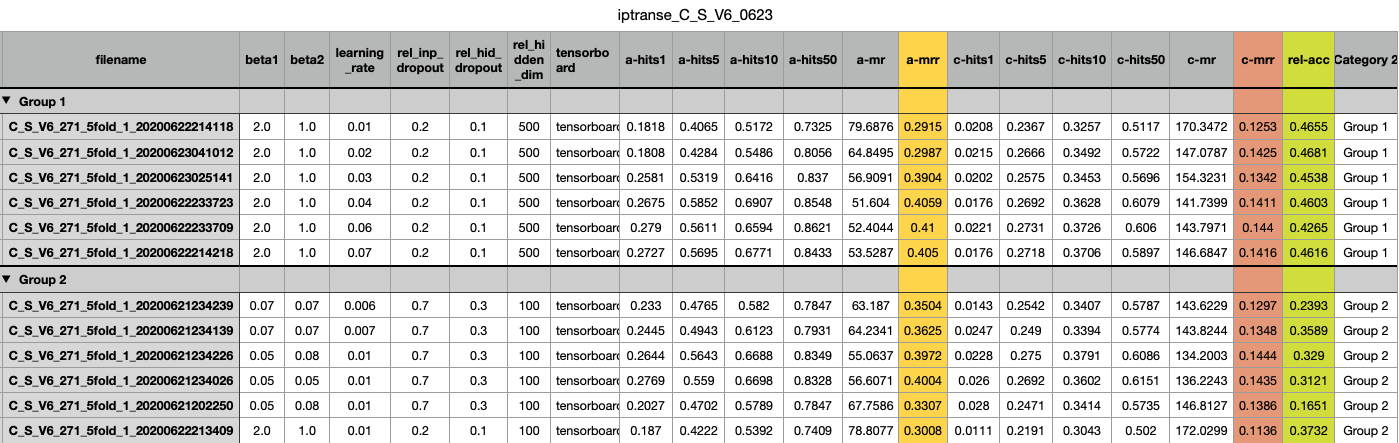
\includegraphics[width=\linewidth]{0623/C_S_V6_0623.png}
    \caption{\label{tab:asynchronously_training_results} Results for asynchronously training on 34 relation types. }
\end{figure}
\begin{figure}[!ht]
    \centering
    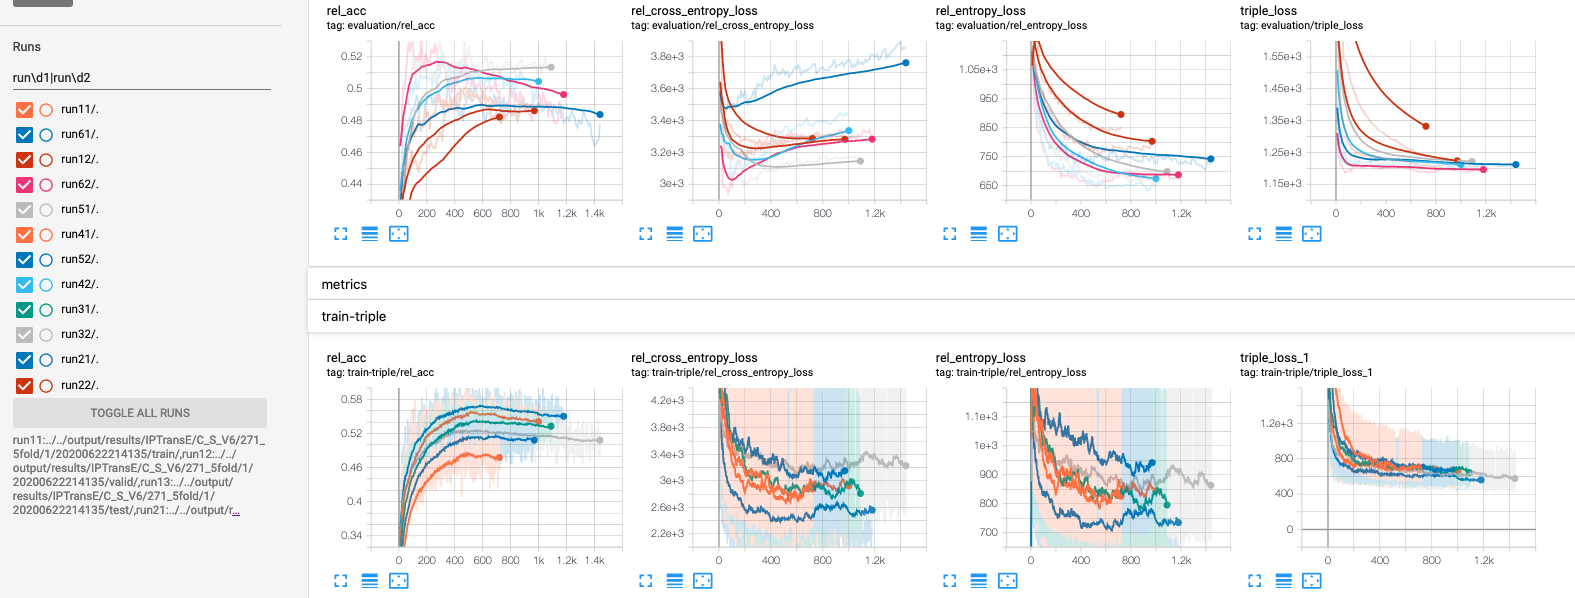
\includegraphics[width=\linewidth]{0623/C_S_V6_0623_learning_curves.png}
    \caption{\label{fig:asynchronously_training_results_curves} Learning curves for Group1 in Figure~\ref{tab:asynchronously_training_results} The top part is the evaluation curves, and the bottom is the training curves (run1* to run6* indicate the learning rate increases from 0.01 to 0.07. (0.05 is still running)).}
\end{figure}
\begin{figure}[H]
    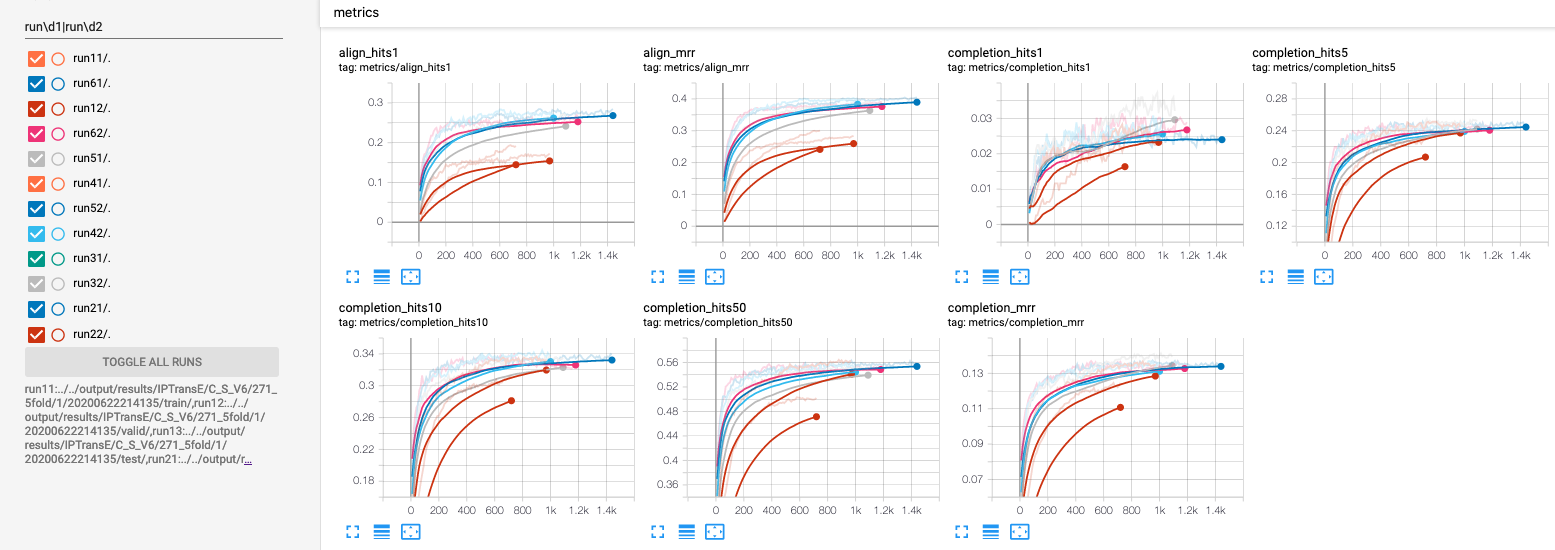
\includegraphics[width=\linewidth]{0623/C_S_V6_0623_metrics_curves.png}
    \caption{\label{fig:asynchronously_metrics_results_curves}  Curves of evaluation metrics for Group1 results in Figure~\ref{tab:asynchronously_training_results} }
\end{figure}

\section{Meeting Notes}


To do list 
\begin{enumerate}
    \item Observe the model outputs on rank, completion, relaiton classification task.
    \begin{enumerate}
        \item Case study: observe head, relation, and tail predictions 
        \item Relation classification confidence measure
        \item Alignment rank confidence measure
        \item Completion rank confidence measure
        \item Visualize the relation labelled SWOW graph. 
    \end{enumerate}
\end{enumerate}

\noindent Possible future directions: Expand to multilingual commonsense knowledge graphs alignment or completion. Becauae both ConceptNet and SWOW has multiple languages version.

\begin{comment}
beta1s=(0.05 0.05 0.05 0.05 0.05 0.05 0.05 0.05) 
beta2s=(0.05 0.08 0.08 0.08 0.08 0.08 0.08 0.05) 
lrs=(0.01 0.007 0.006 0.005 0.004 0.003 0.002 0.001

beta1s=(0.07 0.07 0.07 0.07 0.07 0.07 0.07 0.07) 
beta2s=(0.07 0.07 0.07 0.07 0.07 0.07 0.07 0.07) 
lrs=(0.01 0.007 0.006 0.005 0.004 0.003 0.002 0.001)

tensorboard --logdir=run11:"../../output/results/IPTransE/C_S_V6/271_5fold/1/20200622214135/train/",run12:"../../output/results/IPTransE/C_S_V6/271_5fold/1/20200622214135/valid/",run13:"../../output/results/IPTransE/C_S_V6/271_5fold/1/20200622214135/test/",run21:"../../output/results/IPTransE/C_S_V6/271_5fold/1/20200623041025/train/",run22:"../../output/results/IPTransE/C_S_V6/271_5fold/1/20200623041025/valid/",run23:"../../output/results/IPTransE/C_S_V6/271_5fold/1/20200623041025/test/",run31:"../../output/results/IPTransE/C_S_V6/271_5fold/1/20200623025154/train/",run32:"../../output/results/IPTransE/C_S_V6/271_5fold/1/20200623025154/valid/",run33:"../../output/results/IPTransE/C_S_V6/271_5fold/1/20200623025154/test/",run41:"../../output/results/IPTransE/C_S_V6/271_5fold/1/20200622233738/train/",run42:"../../output/results/IPTransE/C_S_V6/271_5fold/1/20200622233738/valid/",run43:"../../output/results/IPTransE/C_S_V6/271_5fold/1/20200622233738/test/",run51:"../../output/results/IPTransE/C_S_V6/271_5fold/1/20200623072050/train/",run52:"../../output/results/IPTransE/C_S_V6/271_5fold/1/20200623072050/valid/",run53:"../../output/results/IPTransE/C_S_V6/271_5fold/1/20200623072050/test/",run61:"../../output/results/IPTransE/C_S_V6/271_5fold/1/20200622233723/train/",run62:"../../output/results/IPTransE/C_S_V6/271_5fold/1/20200622233723/valid/",run63:"../../output/results/IPTransE/C_S_V6/271_5fold/1/20200622233723/test/",run71:"../../output/results/IPTransE/C_S_V6/271_5fold/1/20200622214236/train/",run72:"../../output/results/IPTransE/C_S_V6/271_5fold/1/20200622214236/valid/",run73:"../../output/results/IPTransE/C_S_V6/271_5fold/1/20200622214236/test/",run81:"../../output/results/IPTransE/C_S_V6/271_5fold/1/20200623061933/train/",run82:"../../output/results/IPTransE/C_S_V6/271_5fold/1/20200623061933/valid/",run83:"../../output/results/IPTransE/C_S_V6/271_5fold/1/20200623061933/test/"
\end{comment}